\chapter{Theory}
\label{chap:theory}

%\chapterquote{The career of a young theoretical physicist consists of treating the harmonic oscillator in ever-increasing levels of abstraction.}{Sidney Coleman}

\newpage

\section{Introduction}
Modern particle theory is built upon the twin pillars of Yang-Mills theories and spontaneous symmetry breaking. 
Our best current model, the Standard Model (SM), is built from two such theories: electroweak theory and quantum chromodynamics. The former of these has its gauge symmetry spontaneously broken. 
In this chapter we will explore these two ideas before moving on to how they are used to construct the SM with particular emphasis on the mechanism of symmetry breaking and one of its phenomenological consequences: the Higgs boson. 

\section{Yang-Mills Theories}
\subsection{From Geometry to Gauge Fields}
The gauge covariant derivative $D_{\mu}$ and the field strength tensor $F_{\mu\nu}$ are two vital mathematical objects when one wants to construct the Lagrangian of a Yang-Mills theory.
Far from simply being an ansatz, they have a deep origin in the fundamental geometry of field theory. 
Their origin is outlined in this section: we start by describing the concept of a fibre bundle, its relationship to the internal symmetries of a field, and how the `warping' of a fibre bundle is related to the covariant derivative and the field strength tensor.

A fibre bundle $\mathcal{B}$ is a space which can be considered to consist of two parts: the base space $\mathcal{M}$ and the fibre $\mathcal{V}$. For each point $p$ in the base space there is an associated copy of the fibre space and these fibres do not intersect. 
In the context of a field one can consider these to be the external and internal spaces respectively. A special case is an ordinary product space where $\mathcal{B}$ is simply the Cartesian product of $\mathcal{M}$ and $\mathcal{V}$, generally one has more warped examples with curvature and less trivial topology. A visual example is given in Figure \ref{fig:theory:fibre_bundle}.
\begin{figure}[h!]
    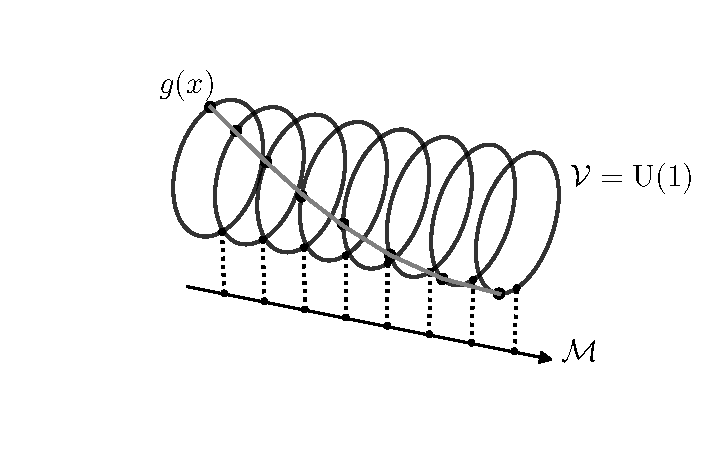
\includegraphics[width=0.5\textwidth]{figures/theory/fibre_bundle.pdf}
    \caption{A fibre bundle with $\mathcal{V} = \mathrm{U}(1)$. A section is shown (grey line) choosing $g(x)\in\mathrm{U}(1)$ for a set of points in $\mathcal{M}$.}
    \label{fig:theory:fibre_bundle}
\end{figure}
These warped examples are of interest in gauge theory, specifically when there is curvature in the fibre space with no torsion.

Particularly, we are interested in the cases when $\mathcal{V}$ is symmetric under some Lie group $\mathcal{G}$ (in our case $\SUN$). 
These symmetries allow for the warping of the fibre bundle and correspond to the internal symmetries of a field. 
Furthermore, one can model these examples by taking the fibre to be $\mathcal{G}$ with the identity element not at a fixed location. 
One can then `lift' the base space into the bundle: for each base space point we get a point within the associated fibre. In the gauge theory context choosing a section of the fibre bundle means choosing a particular $g(x)\in\mathcal{G}$, this is picking a gauge. 

To understand the warping of the fibre bundle we need the notion of a connection just like with the warped spaces of General Relativity.
This will allow for the introduction of warping to the internal space, and construction of invariants such as curvature and torsion tensors.
We can do this by constructing a differential operator $D_{\mu}$, and in our case of a fibre bundle with $\mathcal{V}=\mathcal{G}=\SUN$ where the internal space is simply stretched with no torsion we have,
\begin{equation}
\label{eq:theory:g_connection}
D_{\mu} = \partial_{\mu} - igA_{\mu}^{a} T^{a},
\end{equation}
where $A_{\mu}^{a}$ are generally complex-valued functions that depend on $x_{\mu}$ and operate by multiplying the input, and $T^{a}$ are the generators of the Lie group $\SUN$ which provide a basis in the fibre space with $a = 0,\ldots,N^{2}-1$.
We recognise this as having the familiar form of the gauge covariant derivative and the $A_{\mu}^{a}$ as the gauge potential. 

Now we have the connection we can begin to construct invariants of the geometry of the internal space. In particular we can construct the curvature tensor as follows
\begin{equation}
    \label{eq:theory:g_curvature}
    \frac{i}{g}[D_{\mu},D_{\nu}] = F_{\mu\nu} = \partial_{\mu} A^{b}_{\nu} T^{b} - \partial_{\nu} A^{a}_{\mu} T^{a} - ig[A^{a}_{\mu}T^{a}, A^{b}_{\nu}T^{b}].
\end{equation}
We recognise this form as the field strength tensor.

One can now see what occurs when a global symmetry is promoted to a gauge symmetry: we have induced some non-trivial warping of the field's internal space that gives rise to the $A^{a}_{\mu}$ gauge fields and their kinematics through the curvature $F_{\mu\nu}$.

\subsection{Constructing a Lagrangian}
With these ingredients we can construct a generic Yang-Mills Lagrangian with a straightforward procedure: we begin with a global symmetry of the fields that we promote to a gauge symmetry, we construct the gauge covariant derivative, replace $\partial_{\mu} \rightarrow D_{\mu}$ in the free theory, and add an interaction term based on the field strength tensor. 
As a concrete example, consider the collection of massive free Dirac fermions which we will turn into an interacting gauge theory with $\mathcal{G} = \SUN$.
We first construct the gauge covariant derivative, 
\begin{equation}
    \label{eq:theory:generic_SUN_Dmu}
    D_{\mu} = \partial_{\mu} - igA_{\mu}^{a} T^{a},
\end{equation}
and replace $\partial_{\mu} \rightarrow D_{\mu}$ in the free Lagrangian
\begin{equation}
    \label{eq:theory:int_dirac_no_gauge_dynamics}
    \mathcal{L} = \sum_{\alpha} \bar{\Psi}^{\alpha}[i\gamma^{\mu}(D_{\mu}\Psi)^{\alpha} - m\Psi^{\alpha}].
\end{equation}
We must also introduce a kinematic term for the gauge fields, but the contraction of the general non-Abelian field strength tensor with itself is not gauge invariant, only its trace over the generator indices is. 
We use this as the gauge-invariant kinetic term for our final Yang-Mills Lagranian,
\begin{equation}
    \label{eq:theory:int_dirac_gauge_dynamics}
    \mathcal{L}_{YM} = \sum_{\alpha} \bar{\Psi}^{\alpha}[i\gamma^{\mu}(D_{\mu}\Psi)^{\alpha} - m\Psi^{\alpha}] - \frac{1}{2}\mathrm{Tr}F_{\mu\nu}F^{\mu\nu}.
\end{equation}
%
%

\subsection{Phenomenology}
To analyse what sort of particle interactions occur in this theory we `unpack' equation \ref{eq:theory:int_dirac_gauge_dynamics} and isolate the fields and interaction terms. 
Firstly, in the spectrum of this theory we have $N^{2}-1$ gauge fields (one for each of the generators of $\SUN$) that are all massless. 
These fields couple to the massive fermionic fields via a trilinear interaction term proportional to $g$ introduced by the gauge covariant derivative.
\begin{equation}
    \mathcal{L}_{{A}\Psi} = gA_{\mu}^{a}\bar{\Psi}^{\alpha}\gamma^{\mu}(T^{a})_{\alpha\beta}\Psi^{\beta}
\end{equation}
Now consider the gauge field kinetic term: one can reformulate this as $-\frac{1}{4}F^{a}_{\mu\nu}F^{a\mu\nu}$ using $\mathrm{Tr}T^{a}T^{b} = \frac{1}{2}\delta^{a}_{b}$ and $F_{\mu\nu} = F^{a}_{\mu\nu}T^{a}$. 
Once the product has been evaluated one finds the following forms of interaction terms
\begin{equation}
    \mathcal{L}_{3A} \propto gf^{abc}(\partial_{\mu}v_{\nu\lambda}A^{\lambda{a}})A^{b\mu}A^{c\nu} 
\end{equation}
%
\begin{equation}
    \mathcal{L}_{4A} \propto g^{2}f^{abc}f^{ade}A_{\mu}^{b}A_{\nu}^{c}A_{\lambda}^{d}A_{\sigma}^{e}
\end{equation}
%
that correspond to interactions between three and four gauge bosons respectively. 
We now have the three types of interaction vertices which allow for the construction of Feynman diagrams for a generic Yang-Mills theory (Figure \ref{fig:theory:YM-vertices}). 
Their strengths are all set in terms of a single parameter: the gauge coupling $g$.
One should note that the three and four-gauge boson interactions come from the commutator in the gauge field kinematic term and are not present in the Abelian case. 

\begin{figure}[h!]
    \begin{center}
        \begin{tikzpicture}[baseline=(current bounding box.center)]
        \begin{feynman}
            \vertex (a) {\(A^{a}_{\mu}\)};
            \vertex [right=of a] (b);
            \vertex [above right=of b] (f1) {\(\Psi^{\beta}\)};
            \vertex [below right=of b] (f2) {\(\bar{\Psi}^{\alpha}\)};
            \diagram* {
                (a) -- [boson] (b) -- [fermion] (f1),
                (f2) -- [fermion] (b),
            };
        \end{feynman}
        \end{tikzpicture}
        %
        \qquad
        \begin{tikzpicture}[baseline=(current bounding box.center)]
        \begin{feynman}
            \vertex (a) {\(A^{a}_{\mu}\)};
            \vertex [right=of a] (b);
            \vertex [above right=of b] (f1) {\(A^{b}_{\nu}\)};
            \vertex [below right=of b] (f2) {\(A^{c}_{\lambda}\)};
            \diagram* {
                (a) -- [boson] (b) -- [boson] (f1),
                (b) -- [boson] (f2),
            };
        \end{feynman}
        \end{tikzpicture}
        %
        \qquad
        \begin{tikzpicture}[baseline=(current bounding box.center)]
        \begin{feynman}
            \vertex (b);
            \vertex [above left=of b] (a) {\(A^{a}_{\mu}\)};
            \vertex [below left=of b] (c) {\(A^{b}_{\nu}\)};
            \vertex [above right=of b] (f1) {\(A^{c}_{\lambda}\)};
            \vertex [below right=of b] (f2) {\(A^{d}_{\sigma}\)};
            \diagram* {
                (a) -- [boson] (b), 
                (b) -- [boson] (f1),
                (b) -- [boson] (c),
                (b) -- [boson] (f2),
            };
        \end{feynman}
        \end{tikzpicture}
    \end{center}
    \caption{The three types of vertex in Yang-Mills theories.}
    \label{fig:theory:YM-vertices}
\end{figure}

\section{Spontaneous Symmetry Breaking}
Spontaneous symmetry breaking (SSB) occurs when the lowest energy solutions to a theory do not respect the symmetries of the Lagrangian that describes it. 
A straightforward example is that of a three-dimensional ferromagnetic material cooling down from above its Curie temperature.
Above this threshold there is no magnetisation and solutions obey the $\mathrm{SO}(3)$ symmetry of the Lagranian. 
Below this threshold the ferromagnet becomes magnetised and must `choose' one of a degenerate family of lowest-energy solutions. This picks out a direction of magnetisation. The $\mathrm{SO}(3)$ symmetry of the ferromagnet has now been broken to $\mathrm{SO}(2)$ (Figure \ref{fig:theory:ferromagnet_ssb}).

\begin{figure}[h!]
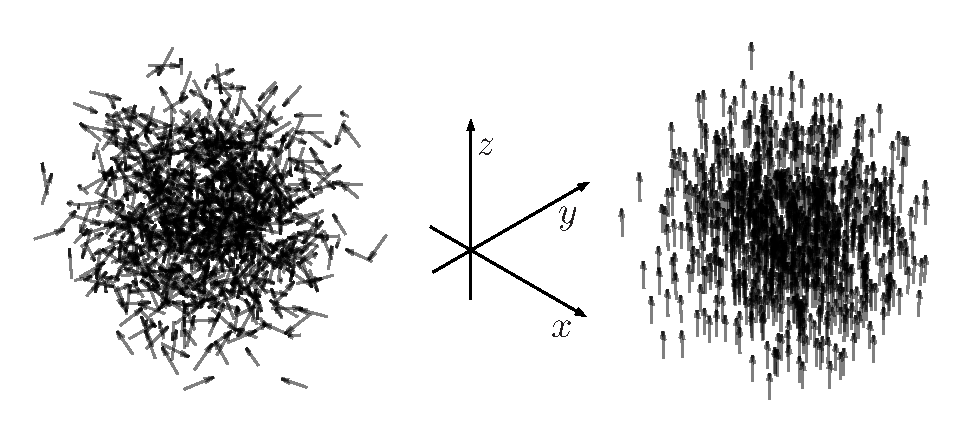
\includegraphics[width=0.8\textwidth]{figures/theory/ferromagnet_ssb.pdf}
\caption{A ferromagnet above (left) and below (right) the Curie temperature. The example below the Curie temperature has magnetised along the z-direction breaking the $\mathrm{SO}(3)$ symmetry to just $\mathrm{SO}(2)$ about the z-axis}
\label{fig:theory:ferromagnet_ssb}
\end{figure}

In the context of a field theory, symmetry can be spontaneously broken in the following way: a field experiences a potential whose minima are a family of degenerate states transforming under the symmetry group. 
Consider the Lagrangian of a complex scalar field $\phi$ experiencing a potential $V(\phi)$,
\begin{equation}
    \label{eq:theory:global_SSB_L}
    \mathcal{L} = (\partial_{\mu}\phi)^{\dag}(\partial^{\mu}\phi) - V(\phi)
\end{equation}
where the potential has the form
\begin{equation}
    \label{eq:theory:global_u1_potential}
    V(\phi) = -\mu^{2}(\phi^{\dag}\phi) + \lambda(\phi^{\dag}\phi)^{2}.
\end{equation}
This has a global $\mathrm{U}(1)$ symmetry, $\phi\rightarrow{e^{i\theta}}\phi$, and the potential has a circle of degenerate minima at $|\phi| = \frac{\mu}{\sqrt{2\lambda}} = v$. 
The vacuum expectation value (VEV) of $\phi$, $\langle\phi\rangle$ is now non-zero and will pick a state in this circle parameterised by $\langle\theta\rangle$ which can take any value $\theta_{0}$. The global symmetry has been spontaneously broken.
\begin{figure}[h!]
    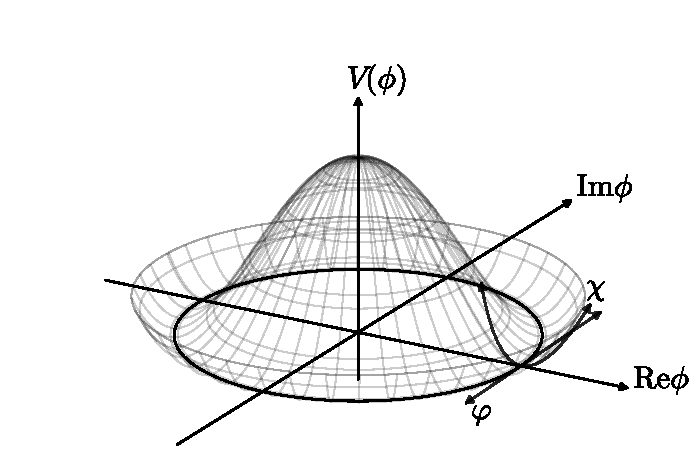
\includegraphics[width=0.5\textwidth]{figures/theory/ssb_potential.pdf}
    \caption{Perturbations around the vacuum state at $\theta_0=0$ of a symmetry breaking potential $V(\phi)$. The family of degenerate minima are shown by the black circle.}
    \label{fig:theory:global_ssb_potential}
\end{figure}
To see the effects of this SSB consider a small perturbation around the vacuum with $\theta_{0}=0$ as shown in Figure \ref{fig:theory:global_ssb_potential}. 
We describe $\phi$ in terms of two real scalar fields: one along the imaginary direction of $\phi$ (along the family of vacuum states) and one along the real (against the potential gradient),
\begin{equation}
    \phi(x) = v + \frac{1}{\sqrt{2}}(\chi(x) + i\varphi(x)).
\end{equation}
If one substitutes this into equation \ref{eq:theory:global_SSB_L} and evaluates the non-kinematic part we find that the field $\chi$ is granted a mass term of the form $\frac{1}{2}m^{2}\chi^{2}$,
\begin{equation}
    \frac{1}{2}m_{\chi}^{2}\chi^{2} = \frac{1}{2}{\lambda}v^{2}\chi^{2}
\end{equation}
and there is no equivalent term for $\varphi$. In the spectrum of this theory we now have a massive and a massless scalar boson upon quantisation. This massless boson is known as a Goldstone boson and is a general result of breaking a global symmetry: for each broken symmetry generator there is a massless Goldstone boson. 

To see this more clearly consider the case of a global $\mathrm{SU}(N)$ symmetry where the Lagrangian has the same form as before (equation \ref{eq:theory:global_u1_potential}) but $\phi$ is now a complex scalar $N$-tuplet. 
There is a global symmetry $\phi\rightarrow{e^{i\theta^{a}T^{a}}}\phi$, and a family of minima at $\phi^{\dag}\phi = \frac{\mu^{2}}{2\lambda}$ that form an $(N^{2}-1)$-dimensional surface instead of a circle. There are $(N^{2}-1)$-many ways to move on this surface and the one remaining direction is away from the centre. The former are the fields associated with the $(N^{2}-1)$ Goldstone bosons and the latter is the single massive scalar boson as before. 

\subsection{Gauge Symmetry Breaking}
In the case where we have a gauge symmetry that is spontaneously broken the behaviour is rather different: there are no Goldstone bosons and the gauge bosons are granted mass. 
To see this take the example of equation \ref{eq:theory:global_SSB_L} and consider a local $\SUN$ symmetry: we construct the gauge-covariant derivative
%
\begin{equation}
    \label{eq:theory:gauge_cov_deriv_u1}
    D_{\mu} = \partial_{\mu} + igA^{a}_{\mu}T^{a},
\end{equation}
%
replace the partial derivative, and introduce a gauge field kinetic term to get the gauge-invariant Lagrangian
\begin{equation}
    \label{eq:theory:gauge_u1_lagrangian}
    \mathcal{L} = (D_{\mu}\phi)^{\dag}(D^{\mu}\phi) - V(\phi) - \frac{1}{2}\mathrm{Tr}F_{\mu\nu}F^{\mu\nu}.
\end{equation}
%
We can consider the field $\phi$ in its ground state in terms of its norm and a local $\SUN$ transformation, and then expand around $v$,
\begin{equation}
    \label{eq:theory:phi_decomposition}
    \phi(x) = e^{i\theta^{a}(x)T^{a}}\begin{pmatrix}
        0\\
        \vdots\\
        v + \frac{1}{\sqrt{2}}H(x)
    \end{pmatrix}
\end{equation}
where $H$ is a real scalar field corresponding to the direction orthogonal to the family of vacua and  the $\theta^{a}$ correspond to the directions along its surface. The fields $\theta^{a}(x)$ now completely parameterise the vacua in contrast to the global case where it was an infinitesimal perturbation around a vacuum state.
As a result of this we recognise that the $\SUN$ transformations can always be removed by some gauge transformation $\exp(-i\theta^{a}(x)T^{a})$, so we can freely set it to zero. 
We have removed $2N-1$ degrees of freedom and we only have only one real scalar left: the gauge freedom has eliminated the Goldstone bosons from the spectrum of the theory.


When we substitute equation \ref{eq:theory:phi_decomposition} with $\theta^{a}(x)=0$ into the Lagrangian \ref{eq:theory:gauge_u1_lagrangian} and then collect the terms that contain $A_{\mu}$ we get the following Lagrangian for the gauge fields (neglecting interaction terms)
\begin{equation}
    \label{eq:theory:abelian_gaugefield_L}
    \mathcal{L}_{A} = -\frac{1}{2}\mathrm{Tr}F_{\mu\nu}F^{\mu\nu} + g^{2}v^{2}A^{a}_{\mu}A^{a\mu}
\end{equation}
This contains mass terms of the form $\frac{1}{2}m_{A}^{2}A_{\mu}A^{\mu}$, so we conclude that the fields $\theta^{a}(x)$ have indeed been eliminated and that these degrees of freedom have been absorbed into the longitudinal components of the gauge fields $A^{a}_{\mu}$ which have been granted mass $m_{A}^{2}=2g^{2}v^{2}$. 


Collecting the scalar field $H$ terms in the same way we have 
\begin{equation}
    \label{eq:theory:abelian_scalar_SSB_L}
    \mathcal{L}_{H} = \frac{1}{2}(\partial_{\mu}H)(\partial^{\mu}H) - \lambda^{2}v^{2}H^{2}% - \frac{1}{sqrt{2}} 
\end{equation}
and we conclude that the theory contains a massive scalar field with $m_{H}^{2} = 2v^{2}\lambda^{2}$ as in the global case. Upon quantisation fields such as $H$ are called Higgs bosons, and these fields have far-reaching consequences for theories of fundamental physics playing a crucial role in the SM by granting mass to all the fundamental field quanta such as electrons and quarks and by breaking part of the gauge symmetry group of the SM. 


\section{The Standard Model of Particle Physics}
The SM is a phenomenologically-motivated theory of fundamental particle interactions consisting of two Yang-Mills theories: one of the unified weak and electromagnetic interaction (electroweak theory) and one of the strong interaction (quantum chromodynamics). This section will treat these in turn using the theoretical machinery presented in previous sections. At the end of this section the resulting Higgs boson and its behaviour will then be discussed. 
\subsection{Electroweak Theory}
The electroweak unification model of Glashow, Weinberg and Salam was the birth of the SM, and our modern understanding of fundamental physics. In this subsection we will begin by constructing the interaction itself as a massless gauge theory and then break its gauge symmetry via the Brout-Englert-Higgs mechanism. We will then move on to introduce the leptonic sector and then the quark sector discussing their dynamical mass generation and properties. 

\subsubsection{Gauge Fields and the Higgs Field}
We begin with a Yang-Mills theory consisting of a complex scalar $\mathrm{SU}(2)$ doublet $\phi$ 
\begin{equation}
    \label{eq:theory:higgs_doublet}
    \phi = \begin{pmatrix}
        \phi^{+} \\
        \phi^{0}
    \end{pmatrix}
\end{equation}
and a global symmetry group $\mathcal{G}=\mathrm{SU}(2)\times\mathrm{U}(1)$ experiencing a potential $V(\phi)$ of the same form as equation \ref{eq:theory:global_u1_potential}. We build the gauge-covariant derivative 
\begin{equation}
    \label{eq:theory:electroweak_cov_deriv}
    D_{\mu} = \partial_{\mu}\mathbb{1} + {ig}W_{\mu}^{a}T^{a} + \frac{ig'}{2}yB_{\mu}\mathbb{1}
\end{equation}
where $W_{\mu}^{a}$ are the gauge fields corresponding to each of the generators of the $\mathrm{SU}(2)$ subgroup of $\mathcal{G}$, the $\tau^{a}$ are the $\mathrm{SU}(2)$ generators (Pauli Matrices), $B_{\mu}$ is the gauge field corresponding to the Abelian subgroup $\mathrm{U}(1)$, and $g$,$g'$ are the gauge couplings corresponding to the $\mathrm{SU}(2)$ and $\mathrm{U}(1)$ respectively. 
The internal field space here has two complex dimensions and the internal geometry corresponds to unit circle in the 2D complex space ($\mathrm{SU}(2)$) warped by a position-dependent complex phase ($\mathrm{U}(1)$).


We construct the following Lagrangian for the complex scalar theory
\begin{equation}
    \label{eq:theory:electroweak_scalar_lagrangian}
    \mathcal{L} = (D_{\mu}\phi)^{\dag}(D_{\mu}\phi) - V(\phi) - \frac{1}{2}\mathrm{Tr}F_{\mu\nu}F^{\mu\nu} - \frac{1}{4}G_{\mu\nu}G^{\mu\nu}
\end{equation}
where $G_{\mu\nu} = \partial_{\mu}B_{\nu} - \partial_{\nu}B_{\mu}$ is the Abelian field strength tensor.
When $\mu^{2} > 0$, $\phi$ adopts a ground state from the family of minima, gains a non-zero vacuum expectation value (VEV) and breaks the $\mathrm{SU}(2)$ subgroup. 
As described previously the $\mathrm{SU}(2)$-associated weak gauge fields will gain mass terms, but there are extra complications. Consider the gauge fields in terms of their physical states $W_{\mu}^{\pm}$
\begin{equation}
    \label{eq:theory:physical_W_states}
    W^{\pm}_{\mu} = \frac{1}{\sqrt{2}}(W^{1}_{\mu}{\mp}iW^{2}_{\mu})
\end{equation}
and the isospin structure of $D_{\mu}$ is shown explicity by writing it in matrix form

\begin{equation}
    \label{eq:theory:explicit_covderiv_ew}
    D_{\mu} = 
    \begin{pmatrix}
        \partial_{\mu} & 0 \\
        0 & \partial_{\mu} \\
    \end{pmatrix} + 
    \frac{ig}{\sqrt{2}}
    \begin{pmatrix}
        0 & W_{\mu}^{+} \\
        W_{\mu}^{-} & 0  \\
    \end{pmatrix} +
    \frac{i}{2}
    \begin{pmatrix}
        gW_{\mu}^{3} + g'yB_{\mu} & 0 \\
        0 & -gW_{\mu}^{3} + g'yB_{\mu} \\
    \end{pmatrix}.
\end{equation}
Note that both the third component of the $\mathrm{SU}(2)$ gauge field and $B_{\mu}$ both multiply a diagonal matrix in the internal isospin space, as a result of this the symmetry breaking pattern is more complex and the two fields will later need to be unmixed. 
If we substitute this expression into the Lagrangian (equation \ref{eq:theory:electroweak_scalar_lagrangian}) and gather terms quadratic in the fields we have,
\begin{equation}
    \label{eq:theory:electroweak_scalar_quad}
    \begin{split}
    \mathcal{L} =& (\partial_{\mu}H)(\partial^{\mu}H) - 4\lambda{v}^{2}H^{2} \\
                 &+ \frac{1}{2}g^{2}v^{2}W_{\mu}^{+}W^{\mu -} \\
                 &+ \frac{1}{4}v^{2}(gW_{\mu}^{3} - g'yB_{\mu})(gW^{\mu 3} - g'yB^{\mu}) \\
                 &- \frac{1}{2}\mathrm{Tr}F_{\mu\nu}F^{\mu\nu} - \frac{1}{4}G_{\mu\nu}G^{\mu\nu} \\
    \end{split}.
\end{equation}
We observe that there is a mass term present for the Higgs field $H$ and the charged weak bosons $W^{\pm}$, however, the quadratic terms for $W^{3}$ and $B$ are `mixed' and we do not have a simple mass term for $W^{3}$ and a massless $B$ field. These fields must be unmixed by performing a rotation in the internal field space 
\begin{equation}
    \begin{split}
    A_{\mu} =& \cos{\theta_{W}}B_{\mu} + \sin{\theta_{W}}W_{\mu}^{3} \\
    Z_{\mu} =& -\sin{\theta_{W}}B_{\mu} + \cos{\theta_{W}}W_{\mu}^{3} \\
    \end{split}
    \label{eq:theory:mass_diag_fields}
\end{equation}
where $\theta_{W}$ is called the weak mixing angle and is defined as $\tan{\theta_{W}} = g'/g$. The field $Z_{\mu}$ now picks up a mass term,
\begin{equation}
    \frac{1}{2} m_{Z}^{2} Z_{\mu} Z^{\mu} = \frac{1}{4}v^{2}(g^{2}+g'{^2})^{2}Z_{\mu}Z^{\mu}
    \label{eq:theory:Z_mass}
\end{equation}
and the field $A_{\mu}$ does not have a mass term. Upon quantisation these are the neutral weak boson, Z, and the photon of electromagnetism.
We can also examine the Abelian part of the gauge covariant derivative with the unmixed fields, 
\begin{equation}
    D_{\mu}^{\mathrm{Abel}} = \partial_{\mu} + ig\sin{\theta_{W}}(T^{3} + \frac{1}{2}y)A_{\mu}
    \label{eq:theory:charge_operator}
\end{equation}
this leads to the interpretation of $T^{3} + \frac{1}{2}y$ as the electromagnetic charge operator where $T^{3}$ is the third component of weak isospin and $y$ is the hypercharge.


We now have four vector bosons and one scalar boson: the three weak bosons of the weak interaction $(W_{\mu}^{\pm},Z_{\mu}^{0})$, the photon $(A_{\mu})$ of the electromagnetic interaction and the Higgs boson $(H)$ with the quantum numbers shown in table \ref{tab:theory:elecroweak_qn_bosons}.
\begin{table}[h!]
\begin{tabular}{ l | c | c | c }
    Particle & Weak isospin third component ($t_{3}$) & Weak hypercharge ($y$) & $Q = t_3 + \frac{y}{2}$ \\
    \hline
    $W^{\pm}$  & $\pm{1}$ & 0 & $\pm1$ \\
    $Z^{0}$    & 0 & 0 & 0 \\
    $\gamma$    & 0 & 0 & 0 \\
    $H$        & $-\frac{1}{2}$ & 1 & 0 \\
\end{tabular}
\caption{Electroweak quantum numbers of the electroweak gauge bosons and the Higgs boson}
 \label{tab:theory:elecroweak_qn_bosons}
\end{table}

\subsubsection{Leptons}
Leptons, fermionic constituents of the SM that interact only via electroweak interactions, must be introduced in a more careful fashion than in equation \ref{eq:theory:int_dirac_gauge_dynamics}. 
Firstly, neutrinos are assumed massless in the SM (but this not the case in nature).
Experiment also demonstrates that neutrinos only interact with left-handed chirality, and that there are processes involving the decay of $W^{-}\rightarrow{}e^{-}+\bar{\nu_{e}}$. Therefore we begin by assigning each lepton and their counterpart neutrino to a weak isodoublet with $T_{3} = \pm\frac{1}{2}$ 
\begin{equation}
    \label{eq:theory:lepton_isodoublets}
    \begin{pmatrix}
        \nu_{e} \\
        e^{-} \\
    \end{pmatrix},
    \begin{pmatrix}
        \nu_{\mu} \\
        \mu^{-} \\
    \end{pmatrix},
    \begin{pmatrix}
        \nu_{\tau} \\
        \tau^{-} \\
    \end{pmatrix}.
\end{equation}
However, the fact that there are no right-handed neutrino interactions necessitates a different structure: we need to split the leptonic isodoublets into left and right-handed versions with the projection operator
\begin{equation}
    \ell_{e} =\begin{pmatrix}
        \nu_{e} \\
        e_{L}^{-}
    \end{pmatrix},
    e^{-}_{L} = \frac{1-\gamma^{5}}{2}e^{-}
\end{equation}
and we note that the $\mathrm{SU}(2)$ gauge symmetry is actually $\mathrm{SU}(2)_{L}$ which denotes operation with the chirality operator along with the elements of the group, and the $L$ subscript has been omitted from the neutrino field as it is assumed that they are only left-handed. 
We can also write the right-handed leptons doublets as
\begin{equation}
    \label{eq:theory:right_handed_leptons}
    \begin{pmatrix}
        \frac{1-\gamma^{5}}{2}\nu_{e} \\
        \frac{1-\gamma^{5}}{2}e^{-}
    \end{pmatrix}=\begin{pmatrix}
        0 \\
        e_{R}^{-}
    \end{pmatrix},
\end{equation}
this transforms as a singlet under $\mathrm{SU}(2)_{L}$ due to the properties of the projection operator. The electroweak quantum numbers of the leptonic families are shown in table \ref{tab:theory:elecroweak_qn_leptons}
\begin{table}[h!]
\begin{tabular}{ l | c | c | c }
    Particle & Weak isospin third component ($t_{3}$) & Weak hypercharge ($y$) & $Q = t_3 + \frac{y}{2}$ \\
    \hline
    $\nu_{e},\nu_{\mu},\nu_{\tau}$  & $\frac{1}{2} $ & $-1$ & $0$ \\
    $\bar{e}_{L},\bar{\mu}_{L},\bar{\tau}_{L}$  & $-\frac{1}{2} $ & $-1$ & $-1$ \\
    $\bar{e}_{R},\bar{\mu}_{R},\bar{\tau}_{R}$  & $0$  & $-2$ & $-1$ \\
\end{tabular}
\caption{Electroweak quantum numbers of the leptons}
 \label{tab:theory:elecroweak_qn_leptons}
\end{table}

To preserve gauge invariance (due to the singlet nature of the right-handed leptons), and to grant mass only to the lower component of the lepton weak isodoublets, mass is granted dynamically via Yukawa couplings. For each isodoublet there is a coupling to the Higgs field $\phi$ of the form
\begin{equation}
    \label{eq:theory:lepton_yukawa}
    g_{f}(\bar{e}_{R}\phi^{\dag}\ell_{e} + \bar{\ell}_{e}\phi{e}_{R}),
\end{equation}
which is invariant under $\mathrm{SU}(2)_{L}$. Upon spontaneous symmetry breaking the Higgs vacuum expectation value generates mass terms and interactions with the Higgs field of the form
\begin{equation}
    \label{eq:theory:lepton_mass_higgs_int}
    g_{f}v(\bar{e}_{R}e_{L} + \bar{e}_{L}e_{R}) + g_{f}(\bar{e}_{R}e_{L}H + \bar{e}_{L}e_{R}H)
\end{equation}
where we recognise the left hand part of the expression as a fermionic mass term with $m_{f} = g_{f}v$, where $g_f$ is the Yukawa coupling strength. The Lagrangian of the leptonic sector of the SM is then
\begin{equation}
    \begin{split}
    \mathcal{L} =& -\frac{1}{2}\mathrm{Tr}F_{\mu\nu}F^{\mu\nu} - \frac{1}{4}G_{\mu\nu}G^{\mu\nu} \\
                 &+ (D_{\mu}\phi)^{\dag}(D_{\mu}\phi) + \mu^{2}(\phi^{\dag}\phi) - \lambda(\phi^{\dag}\phi)^{2} \\
                 &+ i\sum_{f=e,\nu,\tau}(\bar{\ell}_{f}\gamma^{\mu}D_{\mu}\ell_{f} + g_{f}(\bar{f}_{R}\phi^{\dag}\ell_{f} + \bar{\ell}_{f}\phi{f}_{R})) \\
                 &+ i\sum_{f=e,\nu,\tau}(\bar{f}_{R}\gamma^{\mu}D^{Y}_{\mu}f_{R}), \\
    \end{split}
\end{equation}
where $D^{Y}_{\mu}$ denotes the part of the covariant derivative that corresponds to the hypercharge, and $f$ labels lepton generation. 

\subsubsection{Quarks}
To complete the fermionic content of the SM we must include quarks: fermions with fractional electric charge that transform non-trivially under the full SM gauge group. 
In analogy with the leptons we begin by grouping the quarks into three generations of $\mathrm{SU}(2)_{L}$ isodoublets with $T_{3} = \pm\frac{1}{2}$
\begin{equation}
    \label{eq:theory:quark_isodoublets}
    \begin{pmatrix}
        u \\
        d \\
    \end{pmatrix},
    \begin{pmatrix}
        c \\
        s \\
    \end{pmatrix},
    \begin{pmatrix}
        t \\
        b \\
    \end{pmatrix},
\end{equation}
where from left to right and top to bottom we have the up, down, charm, strange, top and bottom quarks. There are also right-handed singlet fields for each flavour of quark. 

The introduction of the electroweak interaction is performed in the same way as before with the introduction of the covariant derivative and the breaking of the $\mathrm{SU}(2)_{L}$ subgroup by the Higgs mechanism. The quantum numbers of the quarks are shown in table \ref{tab:theory:elecroweak_qn_quarks}.
\begin{table}[h!]
\begin{tabular}{ l | c | c | c }
    Particle & Weak isospin third component ($t_{3}$) & Weak hypercharge ($y$) & $Q = t_3 + \frac{y}{2}$ \\
    \hline
    $u,c,t$ & $\frac{1}{2}$ & $\frac{1}{3}$ & $\frac{2}{3}$\\ 
    $d,s,b$ & $-\frac{1}{2}$ & $\frac{1}{3}$ & $-\frac{1}{3}$\\ 
    $u_{R},c_{R},t_{R}$    & $0$ & $\frac{4}{3}$ & $\frac{2}{3}$\\ 
    $d_{R},s_{R},b_{R}$    & $0$ & $-\frac{2}{3}$ & $-\frac{1}{3}$\\ 
\end{tabular}
\caption{Electroweak quantum numbers of the quarks}
\label{tab:theory:elecroweak_qn_quarks}
\end{table}

However, the mechanism for the generating quark masses is slightly different. One still uses couplings of the same form as before, but a few modifications are required to generate masses for the up-type quarks which would remain massless if we proceeded in the exact same way as for leptons. Firstly, note that the following also transforms as an $\mathrm{SU}(2)_{L}$ doublet 
\begin{equation}
    \phi_{C} = i\tau_{2}\phi^{*} = 
    \begin{pmatrix}
        \phi^{0*} \\
        -\phi^{+*}\\
    \end{pmatrix},
    \langle{\phi_{C}}\rangle = 
    \begin{pmatrix} 
        v \\ 
        0 \\ 
    \end{pmatrix},
\end{equation}
where $\tau_{2}$ is the second Pauli matrix. Now, when the Higgs isodoublet gains a vacuum expectation value this transformed version has the value in the upper part of the isodoublet and one can use this to construct gauge-invariant masses for the quarks of the following form
\begin{equation}
    \sum_{i=1,2,3}g_{i}(
    \bar{u}_{iR}\phi^{\dag}q_{iL} 
    + \bar{d}_{iR}\phi^{\dag}_{C}q_{iL}
    + \mathrm{h.c.})
\end{equation}
where h.c. denotes Hermitian conjugate. This grants equal masses to the up and down-type quarks in disagreement with experiment. We therefore have to introduce matrix-valued couplings which mix the flavours
\begin{equation}
    \sum_{i,j=1,2,3}g(
      \alpha_{ij}\bar{u}_{iR}\phi^{\dag}q_{jL} 
      + \beta_{ij}\bar{d}_{iR}\phi^{\dag}_{C}q_{jL}
      + \mathrm{h.c.}).
\end{equation}
Finally, in the physical flavour-changing currents of the SM it is combinations of down type quarks that appear. Each type of quark is measured to have a preference for their own generation but can also decay through the weak interaction to others. We can consider the down-type quarks to be `rotated' in flavour space such that the lower component of the quark isodoublets are actually mixed between $d,s,b$. We therefore replace the down part of each with 
\begin{equation}
    \begin{pmatrix}
        u \\
        d{'} \\
    \end{pmatrix},
    \begin{pmatrix}
        c \\
        s{'} \\
    \end{pmatrix},
    \begin{pmatrix}
        t \\
        b{'} \\
    \end{pmatrix},
    q{'}_{f} = \sum_{f'=d,s,b}V_{ff'}q_{f'}
\end{equation}
where the $V_{ff'}$ are elements of the Cabbibo-Kobayashi-Maskawa (CKM) matrix, a unitary matrix that performs the required rotation in flavour space.

\subsection{Quantum Chromodynamics}
As mentioned previously quarks are the only fermions of the SM to transform non-trivially under the full SM gauge group. This means that they experience an extra interaction from the gauging of the $\mathrm{SU}(3)$ subgroup, the strong interaction, and carry colour charge. This is described by quantum chromodynamics (QCD), the other Yang-Mills theory which constitutes the SM. 

To construct the Lagrangian of QCD we begin by defining the $\mathrm{SU}(3)$ covariant derivative
\begin{equation}
    D_{\mu} = \partial_{\mu} + ig_{s}t^{a}A^{a}_{\mu}
\end{equation}
where $t^{a}$ are the generators of $\mathrm{SU}(3)$, and $g_{s}$ is QCD gauge coupling. Then replace $\partial_{\mu}$ in a Dirac-type Lagrangian that has the corresponding non-Abelian field strength tensor $F^{a}_{\mu\nu}$ and whose fermions are the six flavours of quarks. 
Each of these are isodoublets that also carry the colour charge $q^{C}_{f}$, $C=R,G,B$ (red, green, blue) and are structured in colour triplets transforming under $\mathrm{SU}(3)$
\begin{equation}
    \psi_{f} = \begin{pmatrix}
        q_{f}^{R} \\
        q_{f}^{G} \\
        q_{f}^{B} \\
    \end{pmatrix}.
\end{equation}
The Lagrangian is then
\begin{equation}
    \mathcal{L}_{\mathrm{QCD}} = \sum_{f}i\bar{\psi}_{f}\gamma^{\mu}D_{\mu}\psi_{f} - \frac{1}{2}\mathrm{Tr}F_{\mu\nu}F^{\mu\nu}
\end{equation}
where the index $f$ denotes quark flavour. Upon quantisation we will have eight massless gauge bosons called gluons that couple to quark pairs of the same flavour. 

The strong interaction behaves differently to the weak or electromagnetic interactions: instead of the weakening with distance the strong force increases in strength. An important result of this phenomenon is that colour-carrying particles such as quarks and gluons are confined and can only exist within composite particles called hadrons. This is responsible for the phenomenon of jets in high-energy particle collisions. Jets are cone-shaped sprays of particles where a quark or gluon has been produced, cannot exist freely and then hadronizes. 

We now have the full fundamental particle content of the SM and the couplings between them. Next we will consider how the above is manifested as the phenomenology of the Higgs boson.


\subsection{Higgs boson phenomenology}
The Higgs boson couples directly to every massive particle in the SM: either through the gauge-covariant derivative that gives interactions with the weak gauge bosons, or the Yukawa couplings which cause interaction with the non-neutrino fermions. In this section we will look at how Higgs bosons are created in proton-proton collisions at the Large Hadron Collider, and then how they decay.

\subsubsection{Higgs boson production in proton collisions}
There are four main ways that a Higgs boson can be produced in proton collisions: gluon fusion (ggH), vector boson fusion (VBF), associated production (VH), and top fusion (\ttH) (Figure \ref{fig:theory:higgs_production}). 
\begin{figure}[h!]
    \begin{center}
        \begin{tikzpicture}[baseline=(current bounding box.center)]
        \begin{feynman}
            \vertex (a) {\(H\)};
            \vertex [left=1cm of a] (b);
            \vertex [above left=1cm of b] (c);
            \vertex [below left=1cm of b] (d);
            \vertex [left=1cm of c] (e) {\(g\)};
            \vertex [left=1cm of d] (f) {\(g\)};
            \diagram* {
                (a) -- [scalar] (b),
                (c) -- [fermion,edge label=\(t\)] (b),
                (d) -- [fermion,edge label=\(t\)] (c),
                (b) -- [fermion,edge label=\(t\)] (d),
                (c) -- [gluon] (e),
                (d) -- [gluon] (f)
            };
        \end{feynman}
        \end{tikzpicture}
         \begin{tikzpicture}[baseline=(current bounding box.center)]
             \begin{feynman}
            \vertex (a) {\(H\)};
            \vertex [left=1cm of a] (b);
            \vertex [above left=1cm of b] (c);
            \vertex [below left=1cm of b] (d);
            \vertex [left=1cm of c] (e) {\(q\)};
            \vertex [left=1cm of d] (f) {\(q\)};
            \vertex [above right=1cm of c] (g) {\(q{'}\)};
            \vertex [below right=1cm of d] (h) {\(q{'}\)};
            \diagram* {
                (a) -- [scalar] (b),
                (c) -- [boson,edge label=\(W^{\pm}/Z\)] (b),
                (b) -- [boson,edge label=\(W^{\pm}/Z\)] (d),
                (c) -- [fermion] (g),
                (d) -- [fermion] (h),
                (e) -- [fermion] (c),
                (f) -- [fermion] (d)
            };
        \end{feynman}
        \end{tikzpicture}       
%    \end{center}
%    \begin{center}
        \begin{tikzpicture}[baseline=(current bounding box.center)]
        \begin{feynman}
            \vertex (b);
            \vertex [above left=1cm of b] (a) {\(q\)};
            \vertex [below left=1cm of b] (c) {\(\bar{q}\)};
            \vertex [right=1cm of b] (d);
            \vertex [below right=1cm of d] (e) {\(H\)};
            \vertex [above right=1cm of d] (f) {\(W^{\pm}/Z\)};
            \diagram* {
                (a) -- [fermion] (b),
                (b) -- [fermion] (c),
                (b) -- [boson,edge label=\(W^{\pm}/Z\)] (d),
                (d) -- [scalar] (e),
                (d) -- [boson] (f),
            };
        \end{feynman}
        \end{tikzpicture}
        \begin{tikzpicture}[baseline=(current bounding box.center)]
        \begin{feynman}
            \vertex (a) {\(H\)};
            \vertex [left=1cm of a] (b);
            \vertex [above left=1cm of b] (c);
            \vertex [below left=1cm of b] (d);
            \vertex [left=1cm of c] (e) {\(g\)};
            \vertex [left=1cm of d] (f) {\(g\)};
            \vertex [above right=1cm of c] (g) {\(t\)};
            \vertex [below right=1cm of d] (h) {\(\bar{t}\)};
            \diagram* {
                (a) -- [scalar] (b),
                (b) -- [fermion] (c),
                (d) -- [fermion] (b),
                (c) -- [fermion] (g),
                (h) -- [fermion] (d),
                (e) -- [gluon] (c),
                (f) -- [gluon] (d)
            };

        \end{feynman}
        \end{tikzpicture}
    \end{center}
    \caption{The four main production modes of the Higgs boson at the LHC. Left to right: ggH, VBF, VH and \ttH}
    \label{fig:theory:higgs_production}
\end{figure}
Gluon fusion dominates over the other processes for a Higgs boson of mass $m_{H}=125$\,GeV and proton collisions at $\sqrt{s} = 13$\,TeV with a cross section of 49\,pb. VBF is the second largest with 3.8\,pb, VH is third with 2.3\,pb and \ttH is last with $0.5$\,pb. Although ggH has by far the largest cross-section, the other production modes contain extra objects in their final state aiding the separation of Higgs bosons from events that resemble them. In particular VBF gives rise to two highly energetic jets from the final-state quarks with a large angular separation. 

\subsubsection{Higgs boson decays}
Once produced the Higgs boson is predicted to decay very quickly to pairs of particles. At tree-level it will decay into massive particles in proportion to their masses in two different ways: in the case of particles granted mass through the Yukawa couplings (fermions) the branching ratio will be proportional to the square of the mass, in the case of particles granted mass through the gauge-covariant derivative the branching ratio will be proportional to the fourth power of the mass (weak gauge bosons). 
The Higgs boson can also decay via loop diagrams that have a reduced branching ratio. The prevalence of the main decay modes are summarised in table \ref{tab:theory:higgs_branching_ratios}.
\begin{table}[h!]
\begin{tabular}{ l | c | c | c | c | c | c | c}
    Decay Mode & $b\bar{b}$ & $W^{\pm}W^{\mp*}$ & $gg$ & $\tau\bar{\tau}$ & $c\bar{c}$ & $ZZ^{*}$ & $\gamma\gamma$ \\
    \hline
    Branching ratio & 58.2\% & 21.4\% & 8.2\% & 6.3\% & 2.8\% & 2.6\% & 0.23\% \\
\end{tabular}
\caption{Main branching ratios of the Higgs boson}
 \label{tab:theory:higgs_branching_ratios}
\end{table}

The \Hgg decay (Figure \ref{fig:theory:higgs_gammagamma}) is of particular interest in experimental searches despite its relatively small branching ratio. It has a simple, fully-reconstructed final state with no composite objects such a jets or missing momentum, that causes difficulty in a high-multiplicity hadronic environment such as at the LHC. This decay mode's clean signal lead to it being one of the two channels in which the Higgs boson was discovered in 2012.
\begin{figure}[h!]
    \begin{center}
        \begin{tikzpicture}[baseline=(current bounding box.center)]
        \begin{feynman}
            \vertex (a) {\(H\)};
            \vertex [right=1cm of a] (b);
            \vertex [above right=1cm of b] (c);
            \vertex [below right=1cm of b] (d);
            \vertex [right=1cm of c] (e) {\(\gamma\)};
            \vertex [right=1cm of d] (f) {\(\gamma\)};
            \diagram* {
                (a) -- [scalar] (b),
                (b) -- [fermion,edge label=\(t\)] (c),
                (c) -- [fermion,edge label=\(t\)] (d),
                (d) -- [fermion,edge label=\(t\)] (b),
                (c) -- [photon] (e),
                (d) -- [photon] (f)
            };
        \end{feynman}
        \end{tikzpicture}
        \begin{tikzpicture}[baseline=(current bounding box.center)]
        \begin{feynman}
            \vertex (a) {\(H\)};
            \vertex [right=1cm of a] (b);
            \vertex [above right=1cm of b] (c);
            \vertex [below right=1cm of b] (d);
            \vertex [right=1cm of c] (e) {\(\gamma\)};
            \vertex [right=1cm of d] (f) {\(\gamma\)};
            \diagram* {
                (a) -- [scalar] (b),
                (b) -- [photon,edge label=\(W^{\pm}\)] (c),
                (c) -- [photon,edge label=\(W^{\pm}\)] (d),
                (d) -- [photon,edge label=\(W^{\pm}\)] (b),
                (c) -- [photon] (e),
                (d) -- [photon] (f)
            };
        \end{feynman}
        \end{tikzpicture}
        \begin{tikzpicture}[baseline=(current bounding box.center)]
        \begin{feynman}
            \vertex (a) {\(H\)};
            \vertex [right=1cm of a] (b);
            \vertex [right=1cm of b] (c);
            \vertex [above right=1cm of c] (d) {\(\gamma\)};
            \vertex [below right=1cm of c] (e) {\(\gamma\)};
            \diagram* {
                (a) -- [scalar] (b),
                (b) -- [photon, half left, edge label=\(W^{\pm}\)] (c),
                (c) -- [photon, half left, edge label=\(W^{\pm}\)] (b),
                (c) -- [photon] (d),
                (c) -- [photon] (e),
            };
        \end{feynman}
        \end{tikzpicture}
    \end{center}
    \caption{Main contributing diagrams to the Higgs diphoton decay mode.}
    \label{fig:theory:higgs_gammagamma}
\end{figure}





